\chapter{Resultados e discussões}

Neste capítulo são apresentados os resultados para a biblioteca \emph{PubMed Dataset}, o algoritmo de sumarização \emph{Extraction Engine} e o sistema \emph{BioSearch Refinement}. Os dados utilizados na analise do \emph{PubMed Dataset}, foram utilizados para avaliar o \emph{Extraction Engine} com uma perspectiva diferente.

\section{Resultados do \emph{PubMed Dataset}}
Para a criação dos conjuntos de dados primeiramente foram definidos os termos de busca, o
número máximo de artigos a ser buscado e em seguida foram definidos os atributos dos artigos
que seriam necessários nos conjunto de dados. Cada artigo necessita conter o resumo que será
utilizado para a obtenção das palavras chave geradas pelo algoritmo e também das palavras
chave definidas pelos autores, pois estas são a referência da comparação com as palavras
automaticamente extraídas pelo \emph{Extraction Engine}.

Existem dois tipos de palavras-chave usadas na base de dados do PubMed: os termos de
indexação MeSH e as palavras-chave fornecidas pelos autores do artigo. Os experimentos foram
realizados utilizando como referência os termos MeSH, pois se encontraram poucos artigos com
palavras-chave dos autores.

A biblioteca foi avaliada sob os seguintes aspectos: facilidade de uso (linhas de código para executar a tarefa desejada) e performance (tempo de execução). O objeto de estudo foi a criação de dois conjuntos de dados que seriam utilizados para analisar o \emph{Extraction Engine}, mostrados na Tabela \ref{tab:datasets}.


\begin{table}[htbp]
\center
\begin{tabular}{|l|l|}
\hline
\multicolumn{ 2}{|c|}{\textbf{Conjunto de dados 1}} \\ \hline
Termo de busca & \textit{mycobacterium tuberculosis} \\ \hline
Número de artigos solicitados & \multicolumn{1}{r|}{10000} \\ \hline
Número de artigos recuperados & \multicolumn{1}{r|}{8045} \\ \hline
\multicolumn{ 2}{|c|}{\textbf{Conjunto de dados 2}} \\ \hline
Termo de busca & \textit{h1n1 influenza virus} \\ \hline
Número de artigos solicitados & \multicolumn{1}{r|}{5000} \\ \hline
Número de artigos recuperados & \multicolumn{1}{r|}{2858} \\ \hline
\end{tabular}
\caption{Conjuntos de dados criado com o PubMed Dataset}
\label{tab:datasets}
\end{table}

Para a criação de um conjunto de dados (\emph{dataset}), são necessárias no mínimo 5 linhas de código. O método da Listagem \ref{lst:datasetCreation} recebe o termo de busca e o número de artigos a ser buscado, em seguida, é criada a configuração de \emph{download} com os atributos necessários e o $ArticleDownloader$ com esta configuração. Os atributos são configurados como obrigatórios, ou seja, todos os artigos devem possuir os atributos solicitados e então é feito o \emph{download} dos artigos. Finalmente os artigos são passados para o serializador que os salva em disco com o nome do termo para identificação.

\lstset{caption={Criação de um \emph{DataSet}},label=lst:datasetCreation}
\begin{lstlisting}
public void criarDataSet(String termo, int quantidade) throws IOException{
    DownloadConfiguration config = new DownloadConfiguration(PMID,ABSTRACT,MESH_TERMS);
    ArticleDownloader downloader = new ArticleDownloader(config);
    downloader.setMandatoryAttributes(true);
    List<DynaArticle> downloadedArticles = downloader.getDynaArticles(termo, quantidade);
    DataSet conceptDS = new ConceptDataSet(articles, "mycobacterium tuberculosis");
    DataSetSerializer.serializeDataSet(conceptDS, termo);
}
\end{lstlisting}

Após a criação dos conjuntos de dados, foram executadas duas rotinas implementadas na classe $ConceptDataSet$ que estende $DataSet$. A primeira ($removeSearchTermFromData()$), remove o termo de busca dos conjuntos de palavras-chave geradas e termos MeSH, pois são irrelevantes para o pesquisador já que ele as usou como termo de busca. A segunda rotina ($intersectKws\_Abstract$) desconsidera os termos MeSH que não estão no texto do resumo, pois como o algoritmo avaliado é de extração, só se pode comparar palavras chave extraídas com palavras do próprio resumo.

Como pode-se perceber, a quantidade de artigos recuperados difere da quantidade solicitada. Alguns dos motivos que causaram a redução do número de artigos nos conjuntos de dados foram: alguns artigos no PubMed não possuem os atributos solicitados na configuração de \emph{download}. As rotinas descritas no parágrafo acima causam a exclusão de alguns artigos, quando estes ficam sem palavras-chave geradas ou termos MeSH.

\subsection{Discussão dos resultados do \emph{PubMed Dataset}}

Com a utilização da ferramenta, a construção dos conjuntos de dados aconteceu de maneira
rápida e fácil, bastando apenas especificar os parâmetros iniciais. A utilização do conjunto de
dados se torna muito flexível, pois os seus dados podem ser alterados e gravados novamente,
seja para atualizar as palavras-chave geradas ou algum outro parâmetro.

A partir da Tabela \ref{tab:tempoExecucao}, pode-se observar que, apesar do tempo para download ter sido
consideravelmente grande para 10.000 artigos, esta fase só é executada uma vez, pois o
conjunto de dados é gravado em disco após a execução e sempre vai ser dependente do tráfego
na rede. Pode-se ver que o tempo levado para carregar o conjunto de dados é muito pequeno,
tornando sua utilização muito conveniente para testes. A quantidade de artigos recuperados
varia muito de acordo com os atributos que foram especificados pelo usuário, quanto maior o
numero destes, menos artigos serão recuperados, pois menor será a probabilidade de um artigo
possuir todos os atributos solicitados. A qualidade dos dados recuperados dependerá do que for
disponibilizado no PubMed, pois os conjuntos de dados criados são uma reflexão dos dados
contidos no banco de dados de origem.

\begin{table}[htbp]
\center
\begin{tabular}{|l|l|l|}
\hline
\textbf{Conjunto de dados} & \textbf{Etapas} & \textbf{Tempo de execução} \\ \hline
\multicolumn{ 1}{|c|}{\textbf{1}} & \textit{Download} & 7,45 minutos \\ \cline{ 2- 3}
\multicolumn{ 1}{|l|}{} & Serialização & 2 segundos \\ \cline{ 2- 3}
\multicolumn{ 1}{|l|}{} & Desserialização & 3 segundos \\ \hline
\multicolumn{ 1}{|c|}{\textbf{2}} & \textit{Download} & 3,11 minutos \\ \cline{ 2- 3}
\multicolumn{ 1}{|l|}{} & Serialização & 859 milissegundos \\ \cline{ 2- 3}
\multicolumn{ 1}{|l|}{} & Desserialização & 1 segundo \\ \hline
\end{tabular}
\caption{Desempenho da ferramenta PubMed Dataset na construção dos conjuntos de dados}
\label{tab:tempoExecucao}
\end{table}

Em um ambiente de teste e avaliação, os testes são criados progressivamente e muitas vezes são adicionados casos de teste mais específicos. Dado esse cenário, é óbvio o fato de que os testes são executados diversas vezes. Sem a utilização desta biblioteca, o tempo gasto para a criação dos dados de teste e execução dos testes propriamente ditos levariam um tempo
considerável. Como podemos observar na Tabela \ref{tab:tempoExecucao}, o tempo gasto para o download dos dados é muito grande e também devemos ressaltar que a consistência do conjunto de dados não é garantida visto que os dados retornados pelo PubMed podem variar com o passar do tempo.

\section{Resultados do \emph{Extraction Engine}}

O ponto crucial do \emph{Extraction Engine} é extrair descritores (palavras-chave) válidos para cada artigo, pois se os descritores selecionados localmente são de qualidade, a sumarização dos artigos no processo global será eficiente. Como o processo de extração de descritores é composto por várias etapas, deve ser feita uma avaliação dos resultados de cada uma destas etapas.

A primeira etapa na qual é importante obter resultados confiáveis é a rotulação das palavras de um resumo. Se as classes gramaticais associadas às palavras forem incorretas ou imprecisas, os conceitos também serão gerados incorretamente.  Nesta etapa é utilizado o rotulador MedPost, que possui uma exatidão de 97.43\% segundo \cite{Smith2004}. Conclui-se que as palavras extraídas dos resumos são realmente as que se deseja (\emph{noun chunks}).

A próxima etapa é a obtenção dos conceitos, que são os descritores propriamente ditos. Para determinar a qualidade dos descritores gerados localmente para um artigo pelo \emph{Extraction Engine}, é necessário comparar estes descritores com palavras-chave pré-definidas associadas ao artigo. Estas palavras-chave pré definidas podem ser atribuídas ao artigo pelos autores ou provenientes de alguma outra fonte confiável. 

Existem dois tipos de palavras-chave usadas na base de dados do PubMed: os termos de indexação Medical Subject Headings (MeSH), que são termos de um vocabulário controlado atribuído por especialistas do NLM, e as palavras-chave fornecidas pelos autores do artigo. Os experimentos apresentados a seguir foram avaliados utilizando como referência os termos MeSH, pois se encontraram poucos artigos com palavras-chave atribuídas pelos autores.

Foram criados dois \emph{datasets} com a utilização da biblioteca \emph{PubMed Dataset} apresentada anteriormente. Ambos os \emph{datasets} foram criados com um número máximo de artigos igual a 4.500. Cada conjunto de dados passou por um processo de filtragem descrito a seguir:

\begin{itemize}
    \item dentro do conjunto de artigos inicialmente recuperados, foram excluídos aqueles artigos que não possuíam resumo ou termos MeSH;
    \item foram desconsiderados os termos MeSH que não estavam contidos no resumo;
    \item artigos que ficam sem termos MeSH pela exclusão são retirados do dataset
    \item foi desconsiderada a palavra-chave da busca inicial, no conjunto de palavras-chave geradas e no conjunto de termos MeSH;
\end{itemize}

Os conjuntos de dados resultantes são mostrados na Tabela \ref{tab:datasetsTeste}:

\begin{table}[htbp]
\center
\begin{tabular}{|l|r|}
\hline
\multicolumn{ 2}{|c|}{\textbf{Conjunto de dados 1}} \\ \hline
Termo de busca & \multicolumn{1}{l|}{\textit{mycobacterium tuberculosis}} \\ \hline
Número de artigos solicitados & 4500 \\ \hline
Número de artigos recuperados & 3119 \\ \hline
Adequados para teste & 2773 \\ \hline
\multicolumn{ 2}{|c|}{\textbf{Conjunto de dados 2}} \\ \hline
Termo de busca & \multicolumn{1}{l|}{\textit{h1n1 influenza virus}} \\ \hline
Número de artigos solicitados & 4500 \\ \hline
Número de artigos recuperados & 3487 \\ \hline
Adequados para teste & 2474 \\ \hline
\end{tabular}
\caption{Conjuntos de dados experimentais}
\label{tab:datasetsTeste}
\end{table}

\subsection{Avaliação}
O experimento consistiu na comparação entre as palavras-chave geradas pelo algoritmo (predições) e os termos MeSH obtidos do PubMed. A comparação pode ser feita de duas formas: exata e parcial. A comparação exata ou estrita permite apenas predições positivas de palavras-chave com 100\% de exatidão (que coincidem totalmente), sendo que predições que coincidem parcialmente são consideradas negativas ou erros. 

A metodologia de avaliação parcial seguida neste trabalho é baseada nas propostas de \cite{Chinchor1995} e \cite{Tsai2006}. A avaliação parcial possui dois tipos de avaliação: a avaliação relaxada e a avaliação justa. A avaliação parcial considera as predições que coincidem parcialmente como positivas (similaridade = 1).

Ao fazer comparações com os termos MeSH, resultados parciais podem ser bastante próximos das palavras definidas nos termos MeSH e não devem ser tratadas como erro ou fora do conjunto relevante. A proposta de avaliação parcial justa introduz alguns tipos de resultados parciais que podem ser considerados como resultados positivos próximos por similaridade. Para cada caso, os exemplos fornecidos foram obtidos na execução dos conjuntos de dados.

\begin{itemize}
    \item Coincidência total (Exata): mapeamento completo entre a palavra-chave extraída e a palavra-chave definida manualmente.\\
            \textbf{Termo MeSH}: “rats diseases”\\
            \textbf{Predição}: “rats diseases”
            
    \item Correspondência de sufixo Classe 1: correspondência parcial entre as palavras-chave, que compartilham um sufixo comum. Assume-se que a palavra-chave extraída é um subconjunto do termo manual. Semanticamente, o termo manual é mais específico que a palavra-chave obtida automaticamente.\\
\textbf{Termo MeSH}: “h1n5 influenza virus”\\
\textbf{Predição}: “influenza virus”
    
    \item Correspondência de sufixo Classe 2: correspondência parcial entre as palavras-chave, que compartilham um sufixo comum. Assume-se o contrário da Classe 1, o termo manual é um subconjunto da palavra-chave extraída. Semanticamente, a palavra-chave obtida automaticamente é mais específica que o termo manual.  \\
\textbf{Termo MeSH}: “patients”\\
\textbf{Predição}: “HIV patients”

    \item Correspondência de prefixo Classe 1: correspondência parcial entre as palavras-chave, que compartilham um prefixo comum. Assume-se que o termo manual pode ter um significado diferente que a palavra-chave extraída. Semanticamente, em inglês, a palavra (substantivo) mais à direita define o significado. Portanto, esta classe define que a palavra-chave está contida no prefixo do termo manual.\\
\textbf{Termo MeSH}: “h1n1 influenza virus”\\
\textbf{Predição}: “h1n1 influenza”

    \item Correspondência de prefixo Classe 2: correspondência parcial entre as palavras-chave, que compartilham um prefixo comum. Assume-se que o termo manual pode ter um significado diferente que a palavra-chave extraída. Semanticamente, em inglês, a palavra (substantivo) mais à direita define o significado. Portanto, esta classe define que o termo manual está contido no prefixo da palavra-chave.\\
\textbf{Termo MeSH}: “mycobacterium tb” \\
\textbf{Predição}: “mycobacterium tb infection”

    \item Correspondência por \emph{substring} interno: correspondência parcial de um termo MeSH com uma predição. Ocorre quando um termo MeSH faz parte do interior de uma predição. Assume-se que a predição é mais especializada do que o termo MeSH, ou seja, possui \emph{tokens} a mais. Correspondências de prefixo e sufixo podem ser considerados mais restritos  que a correspondência por \emph{substring} interno. \\
\textbf{Termo MeSH}: “lobe epilepsy”\\
\textbf{Predição}: “temporal lobe epilepsy disease”
\end{itemize}

Nesta avaliação, não foram considerados casos para diferenciar termos em singular e plural, pois tanto os termos MeSH, quanto o algoritmo definem termos no singular.

Cada variação de correspondências parciais vai ser associada a um peso, que corresponde a uma penalidade de acordo com a proximidade por similaridade da palavra-chave extraída do termo manual. Os pesos e penalidades por classe são mostrados na Tabela \ref{tab:pesosSimilaridade}.

\begin{table}[htbp]
\begin{center}
\begin{tabular}{|l|p{3cm}|l|l|l|}
\hline
\multicolumn{1}{|c|}{\textbf{Prioridade}} & \multicolumn{1}{c|}{\textbf{Tipo}} & \multicolumn{1}{c|}{\textbf{Problema}} & \multicolumn{1}{c|}{\textbf{Peso}} & \multicolumn{1}{c|}{\textbf{Penalidade}} \\ \hline
1 & Coincidência \mbox{total} & Nenhum & 1 & 0 \\ \hline
2 & Correspondência de sufixo Classe 1 & Generalização  & 0.9 & 0.1 \\ \hline
3 & Correspondência de sufixo Classe 2 & Especialização  & 0.7 & 0.3 \\ \hline
4 & Correspondência de prefixo Classe 1 & Variação semântica  & 0.5 & 0.5 \\ \hline
5 & Correspondência de prefixo Classe 2 & Variação semântica  & 0.5 & 0.5 \\ \hline
6 & Correspondência substring  & Pode ter variação semântica  & 0.5 & 0.5 \\ \hline
\end{tabular}
\end{center}
\caption{Pesos e penalidades por classe}
\label{tab:pesosSimilaridade}
\end{table}

A modalidade de Sufixo Classe 1 tem a menor das penalidades já que os termos MeSH são uma especificidade do extraído (o extraído é uma generalização do termo MeSH). A Classe 2 do sufixo é o caso contrário, ou seja, o termo MeSH é uma generalização do extraído, o que faz com que a penalidade também seja baixa, mas levando em consideração que está sendo mais específico que o termo sugerido pelos autores.

Quando a penalidade é baixa, o peso é alto. As prioridades definem a preferência de uma palavra extraída para um termo MeSH. Supondo que existem duas palavras extraídas com correspondência para um termo, a preferência vai ser daquela que teve maior prioridade.

Já as modalidades de prefixo podem gerar diferenças semânticas. Para a Classe 1, onde a palavra-chave pode introduzir mudanças semânticas, a penalidade é maior que a anterior e atribui-se um peso e penalidade média, assim também para o caso da modalidade Prefixo Classe 2. Com essas considerações, é possível definir uma ordem parcial que reflita o grau de confiança ao calcular o \emph{recall}, onde 1 significa correspondência total e 0 incompatibilidade total, para aplicar as métricas tradicionais de RI para uma avaliação justa. 

Para avaliar a efetividade dos resultados foram utilizadas as duas métricas mais bem aceitas na comunidade de RI: \emph{precision} e \emph{recall}, além do \emph{F1-measure}.

O número de palavras-chave corretamente extraídas na avaliação justa é calculado como o somatório dos pesos. Assim se temos duas correspondências exatas (1) e uma de Sufixo Classe 1 (0.9) e uma de Prefixo Classe 2 (0.5), o número de correspondências corretas é 3.4. Cada correspondência fica entre 0 e 1. A avaliação aconteceu para cada uma das etapas do algoritmo, focando, principalmente, nas predições da etapa de conceitualização local.

\subsection{Discussão dos resultados do \emph{Extraction Engine}}
A discussão dos resultados é feita para cada conjunto de dados. Na Tabela \ref{tab:dadosDataset} são mostrados alguns dados, relacionados à execução do algoritmo sobre os resumos analisados para cada \emph{dataset}. Para os 2.773 documentos analisados no primeiro \emph{dataset}, o número total de predições foi 24.149 e, na média, oito predições foram extraídas por resumo. Pode-se perceber que o número de predições é 3 vezes maior que o número de termos MeSH, o que irá acarretar um valor menor no \emph{precision}.

\begin{table}[htbp]
\center
\begin{tabular}{|l|c|c|}
\hline
 & \multicolumn{1}{l|}{\textbf{Dataset 1}} & \multicolumn{1}{l|}{\textbf{Dataset 2}} \\ \hline
Número total de artigos analisados & 2773 & 2474 \\ \hline
Número total de predições  & 24149 & 18243 \\ \hline
Número máximo de predições por resumo & 53 & 27 \\ \hline
Número mínimo de predições por resumo & 1 & 1 \\ \hline
Número médio de predições por resumo & 8 & 7 \\ \hline
Número total de termos MESH & 8062 & 6910 \\ \hline
Número máximo de termos MESH por resumo & 14 & 12 \\ \hline
Número mínimo de termos MESH por resumo & 1 & 1 \\ \hline
Número médio de termos MESH por resumo & 3 & 3 \\ \hline
Tempo de processamento médio por artigo & 13.1 ms & 10.3 ms \\ \hline
Tempo de processamento & 24 secs. & 19 secs. \\ \hline
\end{tabular}
\caption{Dados da execução por \emph{dataset}}
\label{tab:dadosDataset}
\end{table}

Nas tabelas a seguir, as predições correspondem aos conceitos extraídos localmente para cada artigo. A Tabela \ref{tab:distribuicaoJusta} mostra a distribuição dos resultados para a avaliação justa, já que ela representa a melhor avaliação dos resultados. A distribuição representa o número de palavras-chave extraídas em cada classe de correspondência. A correlação é o coeficiente de correlação para determinar a relação entre as palavras-chave extraídas distribuídas na classe e os termos MeSH. A razão de predição mostra a relação entre a distribuição por classes das palavras extraídas e o número total de predições.

\begin{table}[htbp]
\begin{center}
\begin{tabular}{|p{3cm}|c|c|c|c|c|c|}
\hline
\multicolumn{ 1}{|c|}{\textbf{Tipo}} & \multicolumn{ 2}{p{3cm}|}{\textbf{Distribuição (Predições por classe)}} & \multicolumn{ 2}{p{3cm}|}{\textbf{Correlação (Distribuição/total de predições)}} & \multicolumn{ 2}{p{3cm}|}{\textbf{Razão de predição (Distribuição/total de termos MeSH)}} \\ \cline{ 2- 7}
\multicolumn{ 1}{|l|}{} & \emph{dataset} 1 & \emph{dataset} 2 & \emph{dataset} 1 & \emph{dataset} 2 & \emph{dataset} 1 & \emph{dataset} 2 \\ \hline
Coincidência total & 316 & 204 & 0,013 & 0,011 & 0,039 & 0,03 \\ \hline
Correspondência de sufixo Classe 1 & 12 & 3 & 0,000 & 0,000 & 0,001 & 0,000 \\ \hline
Correspondência de sufixo Classe 2 & 1329 & 919 & 0,055 & 0,05 & 0,165 & 0,133 \\ \hline
Correspondência de prefixo Classe 1 & 14 & 19 & 0,001 & 0,001 & 0,002 & 0,003 \\ \hline
Correspondência de prefixo Classe 2 & 695 & 760 & 0,029 & 0,042 & 0,086 & 0,11 \\ \hline
Correspondência \emph{substring}  & 1144 & 1593 & 0,047 & 0,087 & 0,142 & 0,231 \\ \hline
\textbf{TOTAL de predições} & 24149 & 18243 & \multicolumn{ 2}{r|}{\textbf{Total de termos MeSH}} & 8062 & 6910 \\ \hline
\end{tabular}
\end{center}
\caption{\emph{Dataset} 1, 2 - Distribuição das correspondências de predições}
\label{tab:distribuicaoJusta}
\end{table}

Pode-se observar que a maior parte das correspondências ocorre por sufixo de classe 2 e por correspondência por \emph{substring}. Isso implica que a maioria das palavras-chave geradas são ou uma especialização do termo MeSH, ou fazem parte deste termo. As predições que possuem mais palavras do que um termo MeSH não são identificadas. Isto pode ser devido a que os termos MeSH vêm de um vocabulário controlado, o que limita o poder de comparação com as predições. A correlação e a razão de predição também se vêm afetadas pelo número grande de predições e poucos termos MeSH no \emph{dataset}.

Os resultados obtidos consideram (1) a avaliação exata, onde todos os casos parciais são considerados negativos e (2) a avaliação relaxada onde se analisam as correspondências parciais como casos positivos e (3) a avaliação justa onde se analisam as correspondências parciais segundo seu peso. Ao executar o \emph{Extraction Engine}, foram calculados os valores das métricas de \emph{precision}, \emph{recall} e \emph{F1-measure} para cada \emph{dataset}. Esses resultados são apresentados na Tabela \ref{tab:resultadosPrecisionRecallEE}.

\begin{table}[htbp]
\center
\begin{tabular}{|l|r|r|r|r|r|r|}
\hline
 & \multicolumn{ 3}{c|}{\textbf{Dataset 1}} & \multicolumn{ 3}{c|}{\textbf{Dataset 2}} \\ \hline
\textbf{Avaliação} & \multicolumn{1}{l|}{\textit{Precision}} & \multicolumn{1}{l|}{\textit{Recall}} & \multicolumn{1}{l|}{\textit{F1-measure}} & \multicolumn{1}{l|}{\textit{Precision}} & \multicolumn{1}{l|}{\textit{Recall}} & \multicolumn{1}{l|}{\textit{F1-measure}} \\ \hline
Exata & 0,035 & 0,396 & 0,064 & 0,03 & 0,302 & 0,054 \\ \hline
Justa & 0,064 & 0,729 & 0,118 & 0,067 & 0,675 & 0,122 \\ \hline
Relaxada & 0,084 & 0,952 & 0,155 & 0,095 & 0,962 & 0,174 \\ \hline
\end{tabular}
\caption{Resultados das três avaliações por dataset}
\label{tab:resultadosPrecisionRecallEE}
\end{table}

Dados estes valores, observa-se que o valor do \emph{precision} é baixo. Isto é explicado ao analisar o cálculo feito utilizando como denominador o conjunto total de predições. A Tabela \ref{tab:dadosDataset} mostra que o número médio de termos MeSH por resumo é três, sendo que o número médio de predições é de sete a oito termos por resumo. O gráfico da Figura \ref{fig:meshVsPredicoes} revela que o número de predições aumenta em relação ao tamanho do resumo. Por outro lado, o número de termos MeSH permanece estável independentemente do tamanho do resumo.

\begin{figure}[h!]
    \center    
    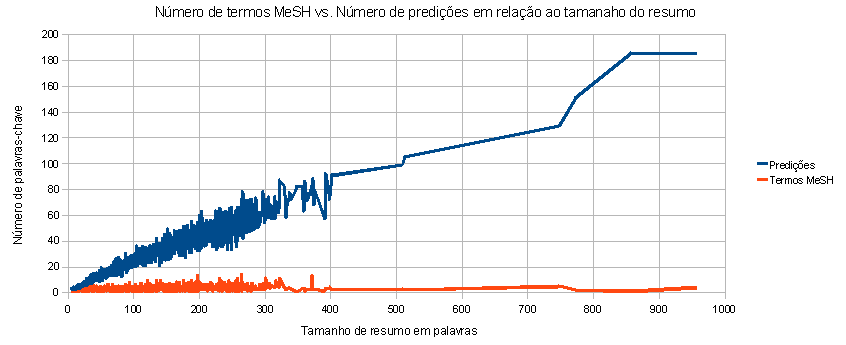
\includegraphics[scale=0.55]{imagens/meshVSpredicoes.png}
    \caption{Número de termos MeSH vs. número de predições em relação ao tamanho em palavras do resumo (para \emph{Dataset} 1)\label{fig:meshVsPredicoes}}
\end{figure}

A Tabela \ref{tab:representacao} mostra as palavras-chave que formam o conjunto global e o número de artigos pertencentes ao conjunto dos documentos recuperados que são indexados pela palavra-chave, assim como a porcentagem que representa dentro do conjunto de documentos. 

\begin{table}[htbp]
\center
\begin{tabular}{|l|p{4cm}|c|c|c|}
\hline
 & \textbf{Palavras-chave globais} & \multicolumn{1}{p{3cm}|}{\textbf{Num. de artigos}} & \multicolumn{1}{p{3cm}|}{\textbf{\% de representação}} & \multicolumn{1}{p{3cm}|}{\textbf{Num. de artigos representados/total de artigos}} \\ \hline
\multicolumn{ 1}{|c|}{Dataset 1} & \textit{mycobacterium tuberculosis} & 173 & 6,2 & 0,062 \\ \cline{ 2- 5}
\multicolumn{ 1}{|l|}{} & \textit{ifn - gamma} & 74 & 2,6 & 0,027 \\ \cline{ 2- 5}
\multicolumn{ 1}{|l|}{} & \textit{t cell} & 55 & 1,9 & 0,02 \\ \cline{ 2- 5}
\multicolumn{ 1}{|l|}{} & \textit{tuberculosis infection} & 55 & 1,9 & 0,02 \\ \cline{ 2- 5}
\multicolumn{ 1}{|l|}{} & \textit{drug resistant} & 52 & 1,8 & 0,019 \\ \hline
\multicolumn{ 1}{|c|}{Dataset 2} & \textit{pandemic influenza a} & 181 & 7,3 & 0,073 \\ \cline{ 2- 5}
\multicolumn{ 1}{|l|}{} & \textit{influenza a} & 168 & 6,7 & 0,068 \\ \cline{ 2- 5}
\multicolumn{ 1}{|l|}{} & \textit{influenza virus} & 98 & 3,9 & 0,04 \\ \cline{ 2- 5}
\multicolumn{ 1}{|l|}{} & \textit{season influenza} & 57 & 2,3 & 0,023 \\ \cline{ 2- 5}
\multicolumn{ 1}{|l|}{} & \textit{acute respiratory distress syndrome} & 36 & 1,4 & 0,015 \\ \hline
\end{tabular}
\caption{Representação do conjunto de palavras-chave global por dataset}
\label{tab:representacao}
\end{table}

Pela tabela acima pode-se observar que cada palavra chave global representa um número reduzido de artigos comparado com a total de artigos retornado, o que facilitaria a busca por temas mais específicos.

\section{Resultados \emph{BioSearch Refinement}}
O mais importante para o sistema como um todo é o tempo de resposta das requisições feitas pelo usuário. Como o \emph{BioSearch Refinement} é um sistema de plataforma \emph{Web}, deve funcionar em um tempo aceitável para um usuário de \emph{Internet}. Para isto, foi feita uma analise da eficiência do sistema como um todo em relação ao tempo de execução.

Os testes de desempenho foram executados em um computador com processador Intel Core 2 Duo, 2.13 Ghz e 3GB de RAM. Como visto na Figura  \ref{fig:fluxoExecucaoEE}, observa-se que o algoritmo \emph{Extraction Engine} está dividido em diversas etapas. A primeira etapa, que é a obtenção dos artigos do servidor PubMed, só depende das condições do próprio servidor e da conexão do usuário, logo o tempo de execução desta parte independe do sistema. O tempo levado em média para obter 1000 artigos do servidor do PubMed foi de 58 segundos. Notou-se que a maior parte do tempo, não é a execução do algoritmo propriamente dito, mas sim a obtenção dos artigos do servidor PubMed. 
Os tempos de execução exibidos na Tabela \ref{tab:temposExecucaoBSR} abaixo são acumulativos das etapas, desde a tokenização de sentenças, PoST, \emph{noun chunking} até a extração global de conceitos ou sumarização. Foram processados 50, 100, 200, 500, 1000 e 2000 artigos de ambos \emph{datasets} com 100\% de extração local de conceitos.

\begin{table}[htbp]
\center
\begin{tabular}{|r|c|c|c|c|c|}
\hline
\multicolumn{1}{|p{3cm}|}{\textbf{Artigos \mbox{processados}}} & \multicolumn{ 5}{l|}{\textbf{Tempo de execução (milissegundos)}} \\ \hline
\multicolumn{1}{|l|}{\textbf{Dataset 1}} & \multicolumn{1}{p{3cm}|}{\textbf{\textit{Part of speech tagging}}} & \multicolumn{1}{l|}{\textbf{\textit{Noun chunking}}} & \multicolumn{1}{p{3cm}|}{\textbf{Conceituali- zação local}} & \multicolumn{ 2}{p{3cm}|}{\textbf{Conceituali- zação global}} \\ \hline
50 & 866 & 898 & 883 & \multicolumn{ 2}{c|}{1043} \\ \hline
100 & 1209 & 1275 & 1214 & \multicolumn{ 2}{c|}{1350} \\ \hline
200 & 2273 & 2217 & 2476 & \multicolumn{ 2}{c|}{2549} \\ \hline
500 & 5966 & 5497 & 6103 & \multicolumn{ 2}{c|}{6231} \\ \hline
1000 & 11391 & 11034 & 11971 & \multicolumn{ 2}{c|}{12380} \\ \hline
2000 & 21737 & 21693 & 23457 & \multicolumn{ 2}{c|}{24376} \\ \hline
\multicolumn{1}{|p{3cm}|}{\textbf{Tempo médio por artigo}} & 11,86 & 10,84 & 11,71 & \multicolumn{ 2}{c|}{-} \\ \hline
\multicolumn{ 6}{|l|}{\textbf{Dataset 2}} \\ \hline
50 & 679 & 757 & 784 & \multicolumn{ 2}{c|}{825} \\ \hline
100 & 960 & 1037 & 1100 & \multicolumn{ 2}{c|}{1146} \\ \hline
200 & 2012 & 2082 & 1977 & \multicolumn{ 2}{c|}{2034} \\ \hline
500 & 4822 & 5096 & 5136 & \multicolumn{ 2}{c|}{5561} \\ \hline
1000 & 9361 & 9885 & 9572 & \multicolumn{ 2}{c|}{10119} \\ \hline
2000 & 18358 & 18616 & 18965 & \multicolumn{ 2}{c|}{19753} \\ \hline
\multicolumn{1}{|p{3cm}|}{\textbf{Tempo médio por artigo}} & 9,17 & 9,38 & 9,48 & \multicolumn{ 2}{c|}{-} \\ \hline
\end{tabular}
\caption{Tempo de execução das etapas do algoritmo}
\label{tab:temposExecucaoBSR}
\end{table}


